\section{What the experiments show}
\begin{frame}[t,label=design]{Synthetic markets}
\small
\setlength{\parskip}{1pt}
The core has 24 clients per side and ten side-exclusive firms, with unit audit
costs. Pairs are feasible within each local market and absent between markets.
\begin{center}
\begin{tabular}{@{}ll@{}}
\toprule
Factor & Values\\
\midrule
Local markets & 1 or 4\\
Rankings & independent or correlated\\
Mean initial exposure & 25\% or 50\%\\
Shared seed blocks & 20\\
\bottomrule
\end{tabular}
\end{center}
$2\times2\times2\times20=160$ markets. Every method sees the same instances.

Partnerships increase exposure odds. A random half of buyers receive
lower exposure odds, independently of preferences.
\sources{All results are synthetic. Lower access is randomly assigned, not a demographic category.
Bootstrap intervals resample whole seed blocks.}
\end{frame}

\begin{frame}[t,label=baselines]{Methods}
\small
\begin{tabularx}{\linewidth}{@{}lX@{}}
\toprule
Method & How it chooses audits\\
\midrule
Three exact variants & Same support model and starting heuristic, different failure cuts.\\[4pt]
Exhaustive search & Check all $2^{10}$ firm-audit vectors.\\[4pt]
Reverse-delete & Start with all firms. Keep a deletion only if DA still passes.\\[4pt]
Blocker greedy & Add the audit with greatest immediate blocker reduction per cost.\\[4pt]
Prefix cover & Expose all prefixes of the full-market DA outcome.\\[4pt]
Full disclosure & Audit every firm.\\
\bottomrule
\end{tabularx}
\sources{Every returned plan passes the DA check. The heuristics have no approximation
guarantee here. The prefix-cover counterexample is in Appendix 6.}
\end{frame}

\begin{frame}[t,label=core]{Results on 160 markets}
\small
\begin{center}
\begin{tabular}{@{}lrrr@{}}
\toprule
Method & Mean cost & At min. & Median (ms)\\
\midrule
Exhaustive search & 4.74 & 160 & 20.8\\
Assignment cuts & 4.74 & 160 & 55.3\\
Component cuts & 4.74 & 160 & 54.7\\
Prefix cuts & 4.74 & 160 & 50.8\\
Reverse-delete & 4.87 & 140 & 1.4\\
Blocker greedy & 5.56 & 62 & 3.9\\
Prefix cover & 4.98 & 126 & 7.4\\
Full disclosure & 10.00 & 0 & ---\\
\bottomrule
\end{tabular}
\end{center}

All exact variants certified every optimum. Reverse-delete usually matched it.
\sources{``At min.'' counts the markets attaining the known optimum (out of 160).
Paired prefix/assignment runtime ratio: 1.007, 95\% interval [0.995, 1.021].
These data show no general speed advantage for prefix cuts.}
\end{frame}

\begin{frame}[t,label=ablation]{The support lower bound}
\small
What happens if we remove the support model? Keep prefix cuts and the same
starting heuristic. Use 40 core markets and a five-second cap.
\begin{center}
\begin{tabular}{@{}lrr@{}}
\toprule
Model & Certified optima & Median seconds\\
\midrule
With support & 40/40 & 0.046\\
Without support & 18/40 & 5.003\\
\bottomrule
\end{tabular}

\end{center}
\medskip
With support, prefix cuts certified 151 of the full 160 markets after
one master solve.

\medskip
The support optimum was strictly below the DA optimum in eight markets,
by one audit each. The other 152 markets had equal optimum costs.
\sources{The 40 markets are a subset of the core sample. The capped median includes timeouts.}
\end{frame}

\begin{frame}[t,label=scale]{Larger markets}
\small
64 clients per side, 24 firms, and a fifteen-second cap.
There are 16 markets in each row below.
\begin{center}
\begin{tabular}{@{}lrrr@{}}
\toprule
Regime & Certified & Median (s) & Max. $U-L$\\
\midrule
One connected market & 9/16 & 9.549 & 2\\
Eight local markets & 16/16 & 0.061 & 0\\
\bottomrule
\end{tabular}

\end{center}
These are prefix-cut results. All three exact variants certified the same
cases. The gap $U-L$ is in audit-cost units.

\medskip
Seven connected cases remained unresolved. A timeout does not tell us
whether the returned plan is suboptimal.
\sources{Every returned plan passed the stability check. Splitting markets also shortens
lists, so the comparison does not isolate the effect of decomposition.}
\end{frame}

\begin{frame}[t,label=stress]{Calls needed to certify the optimum}
\small
Number of three-by-three copies: $N$. Time limit: 10 seconds.
\par\medskip
{\centering
\begin{tabular}{@{}rrrr@{}}
\toprule
$N$ & Assignment cuts & Component cuts & Prefix cuts\\
\midrule
1 & 10 & 3 & 2\\
2 & 131 & 4 & 2\\
3 & \textit{Timeout} & 4 & 2\\
4 & \textit{Timeout} & 5 & 2\\
5 & \textit{Timeout} & 5 & 2\\
6 & \textit{Timeout} & 4 & 2\\
8 & \textit{Timeout} & 7 & 2\\
10 & \textit{Timeout} & 6 & 2\\
\bottomrule
\end{tabular}

\par}
\sources{Timeout: no certificate within 10 seconds. A feasible plan was still returned.
Calls count master solves, excluding initialization.}
\end{frame}

\begin{frame}[t,label=distribution]{Who gains, and who loses?}
\small
Rank score: $0$ if unmatched, otherwise $1-(\mathrm{rank}-1)/(\mathrm{list\ length})$.
\par\centering
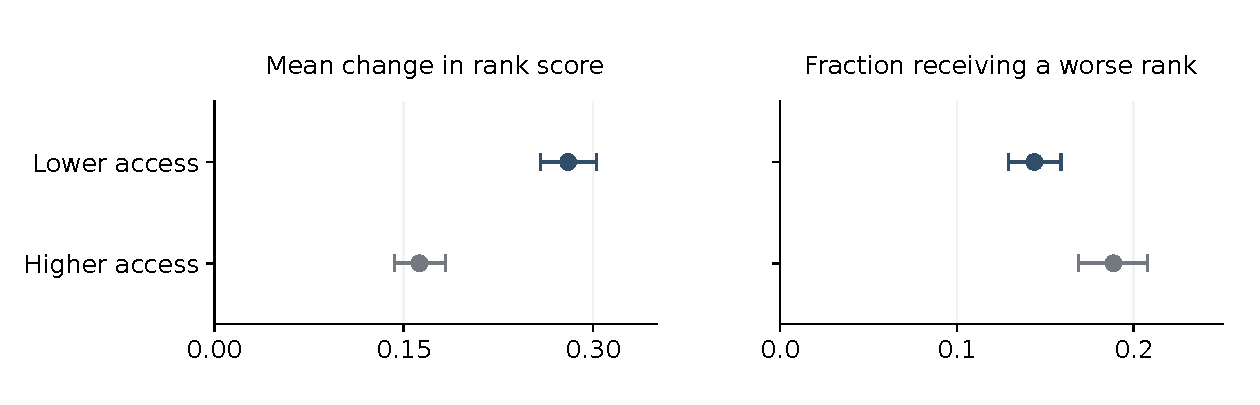
\includegraphics[width=.96\linewidth,height=3.75cm,keepaspectratio]{figures/distribution.pdf}
\par\raggedright
Among lower-access buyers, the selected plans improve mean rank score,
but 14.4\% receive a worse-ranked partner than in the initial DA outcome.
\sources{160 synthetic markets, prefix solver's selected optimal plans.
Intervals are 95\% seed-block bootstrap intervals. Rank score is an ordinal summary,
not welfare. The initial allocation is provisional.}
\end{frame}

\begin{frame}[t,label=ties]{Different optimal plans}
\small
We enumerated all 614 cost-optimal audit plans in the core.
148 markets had multiple optimal plans. In 37, those plans produced
different allocations.
\begin{center}
\begin{tabular}{@{}lr@{}}
\toprule
Every optimal plan worsens at least one\ldots & Markets\\
\midrule
buyer's rank & 155/160\\
seller's rank & 159/160\\
lower-access buyer's rank & 135/160\\
\bottomrule
\end{tabular}
\end{center}
A different cheapest plan can change who loses. It often cannot avoid
individual losses altogether.
\sources{Losses are relative to the initial provisional DA assignment.
These counts do not say that every stable intervention has the same losses.}
\end{frame}
